%% Section 3: IntSeqBERT
%% Japanese draft (draft2/03_model.md) embedded as comments.
%% English translation written below each paragraph.
%% -----------------------------------------------------------------------

\section{IntSeqBERT}
\label{sec:model}

\subsection{Problem Formulation}
\label{sec:formulation}

% OEIS から取り出した整数数列の有限プレフィックスを x = (x_1, ..., x_L)（x_i ∈ Z、L ≤ 128）とする。
% 本研究ではマスク付き系列モデリング（masked sequence modelling）を採用する。位置の一部をランダムに
% マスクし、モデルはマスクされた値を予測するよう学習される。
% 具体的には、マスクされた各位置 i において以下の 3 つの量を予測する：
% 1. Magnitude: v_i（対数スケールの絶対値）
% 2. 符号（Sign）: s_i ∈ {+, -, 0}（3 クラスラベル）
% 3. 剰余（Residues）: 各 m ∈ {2,...,101} に対して r_i^(m) = x_i mod m
% この分解により、大きさ・正負・周期的算術構造が相補的な教師信号として分離される。
Let $\mathbf{x} = (x_1, x_2, \ldots, x_L)$ with $x_i \in \mathbb{Z}$ and $L \leq 128$ be a
finite prefix of an OEIS sequence. We adopt \emph{masked sequence modelling}: a random subset
of positions is masked and the model is trained to predict each masked value. Specifically, for
each masked position $i$, three quantities are predicted:
\begin{enumerate}
  \item \textbf{Magnitude}: $v_i =
    \begin{cases} 0 & (x_i = 0),\\ 1 + \log_{10}|x_i| & (x_i \neq 0) \end{cases} \in \mathbb{R}_{\geq 0}$
  \item \textbf{Sign}: $s_i \in \{+, -, 0\}$ (3-class label)
  \item \textbf{Residues}: $r_i^{(m)} = x_i \bmod m$ for each $m \in \{2, 3, \ldots, 101\}$
        (100 independent classification targets)
\end{enumerate}
This decomposition separates magnitude, sign, and periodic arithmetic structure into
complementary supervision signals.

\subsection{Input Feature Extraction}
\label{sec:features}

% 各要素 x_i について、学習可能な埋め込みの前段で 2 種類の特徴ベクトルを計算する。
% Magnitude 特徴量 f_i^mag ∈ R^4：
%   f_i^mag = [v_i, 1[x_i>0], 1[x_i<0], 1[x_i=0]]
% 後ろ 3 成分は符号（正・負・零）の one-hot 表現である。
% float64 の表現範囲を超える天文学的な整数については、|x_i| の十進桁数でフォールバックする。
% Modulo 特徴量 f_i^mod ∈ R^{200}：
%   各法 m について r = x_i mod m とし、剰余を単位円上の点として埋め込む：
%   φ_m(r) = [sin(2πr/m), cos(2πr/m)] ∈ R^2
%   100 個の法すべてを連結することで f_i^mod ∈ R^{200} を得る。
% この Sin/Cos 埋め込みは Z/mZ の群構造に対して同変であり、折り返し境界での不連続性が生じない。
Two feature vectors are computed for each element $x_i$ prior to learnable embeddings.

\textbf{Magnitude features} $\mathbf{f}_i^{\text{mag}} \in \mathbb{R}^4$:
\[
  \mathbf{f}_i^{\text{mag}} = \bigl[v_i,\;\mathbf{1}[x_i > 0],\;\mathbf{1}[x_i < 0],\;\mathbf{1}[x_i = 0]\bigr].
\]
The last three components are a one-hot sign representation. For astronomically large integers
exceeding the \texttt{float64} range, $|x_i|$ is replaced by its decimal digit count.

\textbf{Modulo features} $\mathbf{f}_i^{\text{mod}} \in \mathbb{R}^{200}$:
For each modulus $m \in \{2, \ldots, 101\}$, let $r = x_i \bmod m$, and embed the residue as
a point on the unit circle:
\[
  \phi_m(r) = \left[\sin\!\left(\tfrac{2\pi r}{m}\right),\;\cos\!\left(\tfrac{2\pi r}{m}\right)\right] \in \mathbb{R}^2.
\]
Concatenating all 100 moduli gives $\mathbf{f}_i^{\text{mod}} \in \mathbb{R}^{200}$.
This Sin/Cos embedding is equivariant to the group structure of $\mathbb{Z}/m\mathbb{Z}$ and
avoids discontinuities at wrap-around boundaries.

\subsection{Dual-Stream Embedding}
\label{sec:dualstream}

% 2 つの特徴ベクトルは独立した射影層でモデルの隠れ次元 d に写像される。
% Magnitude 側に 2 層 MLP を用いる：
% h_i^mag = MLP_mag(f_i^mag),  h_i^mod = W_mod f_i^mod + b_mod,  h_i^mag, h_i^mod ∈ R^d.
The two feature vectors are projected to the model hidden dimension $d$ by independent
projection layers. A two-layer MLP is used for the Magnitude side:
\[
  \mathbf{h}_i^{\text{mag}} = \mathrm{MLP}_{\text{mag}}\!\left(\mathbf{f}_i^{\text{mag}}\right),
  \quad
  \mathbf{h}_i^{\text{mod}} = W_{\text{mod}}\,\mathbf{f}_i^{\text{mod}} + \mathbf{b}_{\text{mod}},
  \quad \mathbf{h}_i^{\text{mag}},\,\mathbf{h}_i^{\text{mod}} \in \mathbb{R}^d.
\]

\subsection{FiLM Fusion}
\label{sec:film}

% 2 つのストリームを Feature-wise Linear Modulation（FiLM）[cite:perez2018film] で融合する。
% Modulo 埋め込みが要素ごとのスケール γ_i とシフト β_i を生成し、Magnitude 埋め込みを変調する：
%   γ_i = W_γ h_i^mod,  β_i = W_β h_i^mod
%   e_i = (1 + γ_i) ⊙ h_i^mag + β_i
% Modulo 側の射影後に ReLU を適用し、さらに FiLM 前にドロップアウトを入れる。
% この定式化により、算術的周期性がパラメータ効率よく連続値の Magnitude 表現を条件付けることができる。
% エンコーダへの入力前に、e_i に標準的な Sin/Cos 位置エンコーディングを加算する。
The two streams are fused by Feature-wise Linear Modulation
(FiLM)~\cite{perez2018film}. The Modulo embedding generates element-wise scale $\boldsymbol{\gamma}_i$
and shift $\boldsymbol{\beta}_i$ to modulate the Magnitude embedding:
\[
  \boldsymbol{\gamma}_i = W_\gamma\,\mathbf{h}_i^{\text{mod}},
  \quad
  \boldsymbol{\beta}_i = W_\beta\,\mathbf{h}_i^{\text{mod}},
\]
\[
  \mathbf{e}_i = (1 + \boldsymbol{\gamma}_i) \odot \mathbf{h}_i^{\text{mag}} + \boldsymbol{\beta}_i.
\]
A ReLU is applied after the Modulo projection, and dropout is inserted before FiLM. This
formulation allows arithmetic periodicity to condition continuous-value Magnitude representations
with parameter efficiency ($W_\gamma, W_\beta \in \mathbb{R}^{d \times d}$). Standard
sinusoidal positional encodings are added to $\mathbf{e}_i$ before the encoder.

The overall architecture is illustrated in Fig.~\ref{fig:architecture}: each element is
projected independently via the Magnitude stream (blue) and the Modulo stream (orange), fused
by FiLM, and passed to the Transformer encoder.

\begin{figure}[t]
  \centering
  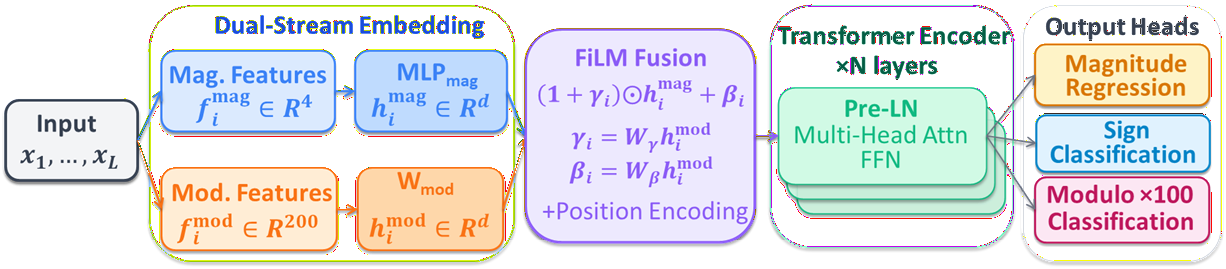
\includegraphics[width=\linewidth]{figures/fig1_architecture}
  \caption{IntSeqBERT architecture. The Dual-Stream Embedding block projects
           $\mathbf{f}^{\mathrm{mag}}\!\in\!\mathbb{R}^4$ and
           $\mathbf{f}^{\mathrm{mod}}\!\in\!\mathbb{R}^{200}$ each to $\mathbb{R}^d$ and
           fuses them via FiLM. Positional encodings are added to the fused embedding before
           the Pre-LN Transformer encoder, which outputs to three prediction heads
           (magnitude regression, sign classification, $100\times$ Modulo classification).}
  \label{fig:architecture}
\end{figure}

\subsection{Transformer Encoder}
\label{sec:encoder}

% 融合された系列を Pre-Layer Normalisation [cite:xiong2020layer] を採用した標準 Transformer
% エンコーダ [cite:vaswani2017attention] で処理する。
% 3 つのモデルサイズで実験を行う：Small (6L, d=256, 4h, 6.4M), Middle (8L, d=512, 8h, 29.0M),
% Large (12L, d=768, 12h, 91.5M)
The fused sequence $(\mathbf{e}_1, \ldots, \mathbf{e}_L)$ is processed by a standard
Transformer encoder~\cite{vaswani2017attention} with Pre-Layer Normalisation~\cite{xiong2020layer}.
Three model sizes are evaluated:

\begin{table}[t]
\caption{Model configurations.}
\label{tab:models}
\centering
\begin{tabular}{lcccr}
\hline
Config  & Layers & $d$ & Heads & Parameters \\
\hline
Small   & 6      & 256 & 4     & 6.4M       \\
Middle  & 8      & 512 & 8     & 29.0M      \\
Large   & 12     & 768 & 12    & 91.5M      \\
\hline
\end{tabular}
\end{table}

\subsection{Prediction Heads}
\label{sec:heads}

% マスク位置 i のエンコーダ出力を z_i ∈ R^d とする。
% Magnitude ヘッド（回帰）：
%   (μ_i, log σ_i^2) = MLP_mag-head(z_i)、予測値は v_hat_i = μ_i
%   MLP_mag-head は隠れ次元 d・活性化 ReLU の 2 層 MLP（d → d → 2）
%   損失計算では主に μ_i を使用し、log σ_i^2 は補助出力として保持する。
% 符号ヘッド（3 クラス分類）：
%   s_hat_i = softmax(W_sign z_i)、W_sign ∈ R^{3×d}
% Modulo ヘッド（独立した m 値分類器 × 100）：
%   各法 m について {0,...,m-1} 上のロジットを出力する線形層。
%   総出力次元 = Σ_{m=2}^{101} m = 5,150
Let $\mathbf{z}_i \in \mathbb{R}^d$ be the encoder output at masked position $i$.

\textbf{Magnitude head} (regression): A two-layer MLP ($d \to d \to 2$, ReLU activation)
outputs $(\mu_i, \log \sigma_i^2)$; the prediction is $\hat{v}_i = \mu_i$.

\textbf{Sign head} (3-class classification):
$\hat{s}_i = \operatorname{softmax}(W_{\text{sign}}\,\mathbf{z}_i)$, $W_{\text{sign}} \in \mathbb{R}^{3 \times d}$.

\textbf{Modulo head} (100 independent classifiers): For each $m \in \{2, \ldots, 101\}$, a
linear layer outputs logits over $\{0, \ldots, m-1\}$ sharing the same input $\mathbf{z}_i$
but with independent parameters. The total output dimension is $\sum_{m=2}^{101} m = 5{,}150$.

\subsection{Training Objective}
\label{sec:training}

% マルチタスク損失：
%   L = w_mag L_mag + w_sign L_sign + w_mod L_mod
%   w_mag = 1.0, w_sign = 1.0, w_mod = 2.0
% 不確実性に基づく動的重み付けは学習不安定化のため採用せず、固定値を採用。
% L_mag: Huber 損失（Smooth L1）
% L_sign: 3 クラスのクロスエントロピー損失
% L_mod: 100 個の Modulo ヘッドのクロスエントロピーの平均（log m 正規化）：
%   L_mod = (1/100) Σ_{m=2}^{101} (1/log m) L_CE^(m)
% すべての損失はマスク位置のみで計算する。
The multi-task loss is:
\[
  \mathcal{L} = w_{\text{mag}}\,\mathcal{L}_{\text{mag}}
              + w_{\text{sign}}\,\mathcal{L}_{\text{sign}}
              + w_{\text{mod}}\,\mathcal{L}_{\text{mod}},
\]
with $w_{\text{mag}} = 1.0$, $w_{\text{sign}} = 1.0$, $w_{\text{mod}} = 2.0$ (fixed; adaptive
weighting based on uncertainty caused instability in preliminary experiments).
$\mathcal{L}_{\text{mag}}$ is Huber loss (Smooth L1) between $\hat{v}_i$ and $v_i$.
$\mathcal{L}_{\text{sign}}$ is cross-entropy over three sign classes.
$\mathcal{L}_{\text{mod}}$ is the mean cross-entropy of the 100 Modulo heads, normalised by
$\log m$ to correct for varying numbers of classes:
\[
  \mathcal{L}_{\text{mod}} = \frac{1}{100}\sum_{m=2}^{101}\frac{1}{\log m}\,\mathcal{L}_{\text{CE}}^{(m)}.
\]
All losses are computed only at masked positions.

\subsection{Baselines}
\label{sec:baselines}

% Vanilla Transformer: 各整数を 20,003 エントリの語彙（0〜19,999 の 20,000 値 + PAD, MASK, UNK）
% のトークン ID に変換する。語彙外の値は UNK で置換。同じ 3 つの予測ヘッドを使用。
% 語彙サイズ 20,003 は VRAM 8 GB 制約の下で IntSeqBERT と同等のメモリ消費となるよう設定。
% アブレーション（Magnitude-only）: IntSeqBERT と同一だが Magnitude ストリームのみを使用し、
% FiLM モジュールを取り除いて e_i = h_i^mag とする。Modulo ストリームの寄与を単独で定量化できる。
\textbf{Vanilla Transformer} maps each integer to a token ID in a vocabulary of 20,003 entries
(values 0--19{,}999 plus \texttt{PAD}, \texttt{MASK}, \texttt{UNK}); out-of-vocabulary values
are replaced by \texttt{UNK}. The same three prediction heads are applied to the token
embeddings. The vocabulary size 20,003 was chosen so that memory consumption matches
IntSeqBERT under the 8\,GB VRAM constraint. The prior benchmark FACT~\cite{zurich-fact}
handles values up to several million, presupposing larger compute resources than our setting.

\textbf{Ablation (Magnitude-only)} is identical to IntSeqBERT but uses only the Magnitude
stream; the FiLM module is removed and $\mathbf{e}_i = \mathbf{h}_i^{\text{mag}}$. This
isolates the contribution of the Modulo stream.

\subsection{IntegerSolver}
\label{sec:solver}

% Solver はまず、Magnitude 予測から 3σ 区間 [n_min, n_max] を導出し、探索範囲の広さ Δn に応じて
% 以下の 3 モードを動的に選択する。
% 符号予測が零の場合は即時に 0 を返す。
% 各候補 n のスコア：
%   score(n) = -(v_n - μ_i)^2 / (2σ_i^2) + 0.3 × Σ_{m=2}^{101} log P(n mod m)
%   係数 0.3 は法間の情報重複でスコアが過大になりやすいことを抑えるための経験的ハイパーパラメータ。
% 上位 k 件の候補を返し、Solver Top-k として評価する。
The pre-trained model outputs Magnitude $(\mu_i, \log \sigma_i^2)$, sign, and Modulo
distributions at masked positions. \textbf{IntegerSolver} recovers concrete integers from these
predictions.

The Solver derives the $3\sigma$ interval $[n_{\min}, n_{\max}]$ from the Magnitude prediction
and dynamically selects one of three modes based on the search width
$\Delta n = |n_{\max} - n_{\min}|$:

\begin{table}[t]
\caption{Solver operating modes.}
\label{tab:solver}
\centering
\begin{tabular}{llp{5.5cm}}
\hline
Mode     & Condition                              & Method \\
\hline
Dense    & $\Delta n \leq 10^6$                   & Enumerate all integers in range \\
Sieve    & $10^6 < \Delta n \leq 10^{14}$         & CRT beam search anchored on high-confidence moduli \\
CRT      & $\Delta n > 10^{14}$                   & Sparse CRT beam search to generate large integers directly \\
\hline
\end{tabular}
\end{table}

When the sign prediction is zero, the Solver immediately returns 0. If no valid candidate is
found in the search range, the call is recorded as \texttt{none}.

Each candidate $n$ is scored as a weighted sum of the Magnitude term and the log-probabilities
over all moduli:
\[
  \text{score}(n) =
  -\frac{(v_n - \mu_i)^2}{2\sigma_i^2}
  + 0.3 \cdot \sum_{m=2}^{101} \log P\!\left(n \bmod m\right),
\]
where $v_n = 1 + \log_{10}|n|$ ($n \neq 0$) or $0$ ($n = 0$). The coefficient 0.3 is an
empirical hyperparameter that suppresses score inflation due to information overlap between
composite and prime moduli. The top $k$ candidates are returned and evaluated as
Solver Top-$k$ accuracy (Section~\ref{sec:solver-eval}).
